\chapter{Results}

The velocity $ v $ of the stream flowing over the sensor is approximately \unitfrac[1]{m}{s}. This allows us to create a relation \eqref{eq:resv} between the spacial resolution $ \diff s $ and the time resolution $ \diff t $.

\begin{equation}
	v = \dfrac{\diff s}{\diff t}
\label{eq:resv} 
\end{equation}

For example, a spacial resolution of \unit[1]{cm} would require a time resolution of \unit[0.01]{s}. However, this assumes the size $ l $ of the sensor and the time $ \tau $ a measurement takes to be infinitesimal small, while in reality it is not. While the sensors measures, the flow continuous and instead of measuring the conductivity of a certain volume at a certain time, an average is measured. Figure \ref{fig:cv} visualizes this issue.

\begin{figure}
	\begin{center}
		\begin{tikzpicture}
		\node [minimum height=32pt, minimum width=32pt, style=rect] (0) at (0, 0) {};
		\draw (-0.55,0) -- (-0.55,-1.5);
		\draw (0.55,0) -- (0.55,-1.5);
		\draw [darrow] (-0.55,-1.3) -- (0.55,-1.3) node[above, pos=0.5] {$l$};

		\node [minimum height=32pt, minimum width=32pt, style=vol] (0) at (-1.5, 0) {};
		\draw [arrow] (-2.05,1) -- (-1,1) node[above, pos=0.5] {$v$};

		\node [] at (4,0) {$t<0$};

		\node [minimum height=32pt, minimum width=32pt, style=rect] (0) at (0, -2.5) {};
		\node [minimum height=32pt, minimum width=32pt, style=vol] (0) at (-0.25, -2.5) {};

		\node [] at (4,-2.5) {$t=0$};

		\node [minimum height=32pt, minimum width=32pt, style=rect] (0) at (0, -4) {};
		\node [minimum height=32pt, minimum width=32pt, style=vol] (0) at (0.25, -4) {};

		\node [] at (4,-4) {$t=\tau$};		
		
		\node [minimum height=32pt, minimum width=32pt, style=rect] (0) at (0, -6) {};
		\node [minimum height=32pt, minimum width=32pt, style=vol] (0) at (1.5, -6) {};
		
		\node [] at (4,-6) {$t>\tau$};
		\end{tikzpicture}
		%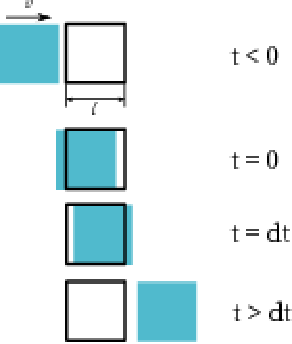
\includegraphics[width=0.45\textwidth]{images/resolution.pdf} 
		\caption{control volume moving over sensor}
		\label{fig:cv}
	\end{center}
\end{figure}

To accommodate for that, factors $ n $ \eqref{eq:resn} and $ k $ \eqref{eq:resk} are introduced, describing the ratio of the resolutions to the actual sizes.

\begin{equation}
	n = \dfrac{l}{\diff s}
\label{eq:resn} 
\end{equation}

\begin{equation}
	k = \dfrac{ \tau}{\diff t}
\label{eq:resk}
\end{equation}

Inserting $ k $ and $ n $ in formula \eqref{eq:resv} yields

\begin{equation}
	v = \dfrac{\diff s}{\diff t} = \dfrac{k \cdot l}{n \cdot \tau}
\label{eq:resv1} 
\end{equation}

The ratio $ r $
\begin{equation}
	r = \frac{k}{n}
\label{eq:resr} 
\end{equation}
is the ratio of the time it takes a control volume to enter and leave the sensor area  to the time a measurement takes. To avoid a smearing of the measurement over multiple control volumes, $ r $ should be 10. This can be achieved with a sensor that has a size $ l $ of \unit[1]{cm}, and a measurement time $ \tau $ of \unit[1]{ms}.

\section{Verification}

Test for each requirement.

\subsection{Time Resolution}

Test if smaller then \unit[1]{ms}.

\subsection{Spacial Resolution}

Inspect if smaller then \unit[1]{cm}. [physical size of sensor is 1 cm, sensor can be directly next to each other. show via drawing]

\subsection{Electrical Conductivity Resolution}

Test if able to distinguish liquids with a conductivity of \unitfrac[5]{S}{m} and \unitfrac[5e-3]{S}{m}.

\subsection{Cost}

Analyse if less than \euro{10} per sensor.

\subsection{Deployment}

Demonstrate that deployable in the algae reactor.

\subsection{Usability}

Test if easy to use by anybody with only a minimal set of written instructions. [find a victim to try to perform a measurement with only written instructions provided]

\section{Validation}

Check, if Timm can use it to measure flow and compare with simulation. [?]

\begin{figure}
	\begin{center}
		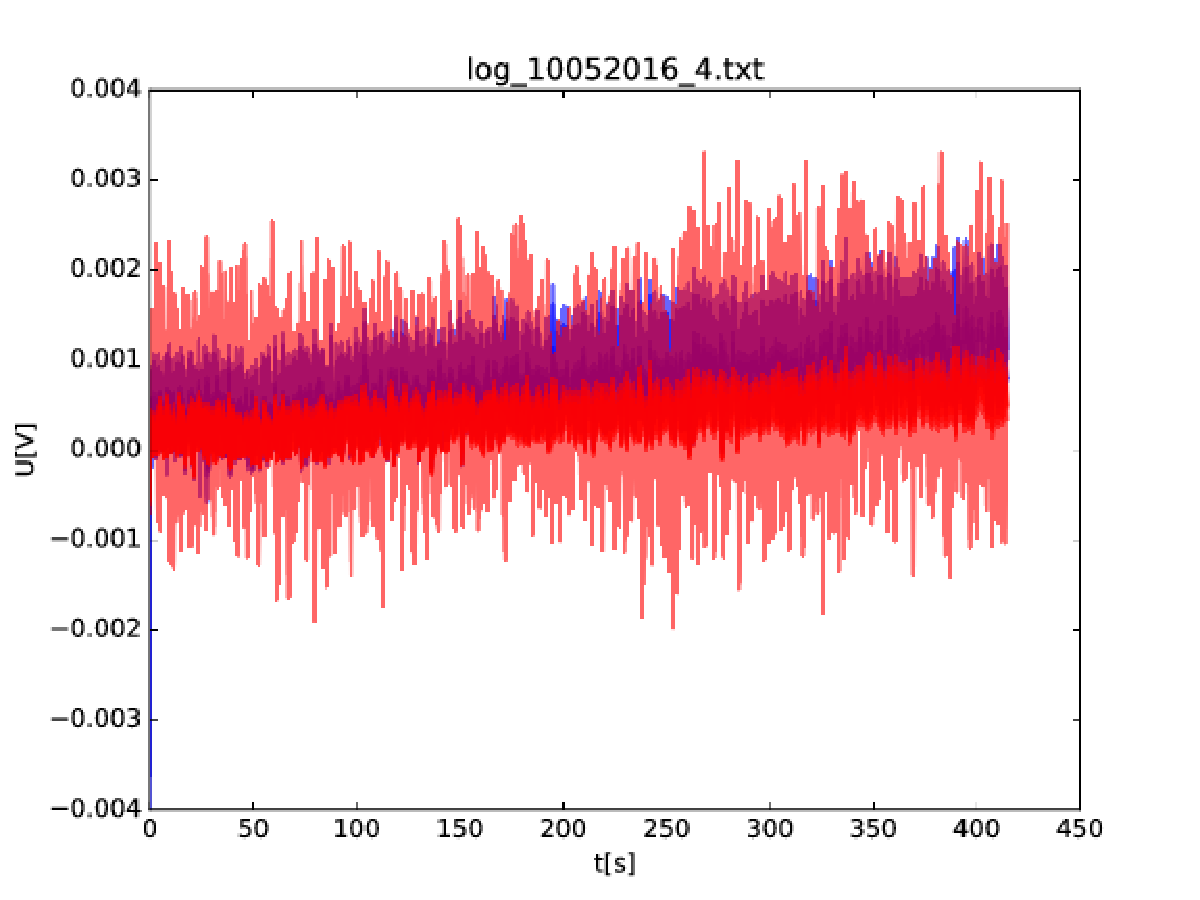
\includegraphics[width=\textwidth]{images/noise.pdf} 
		\caption{noise}
	\end{center}
\end{figure}

\begin{figure}
	\begin{center}
		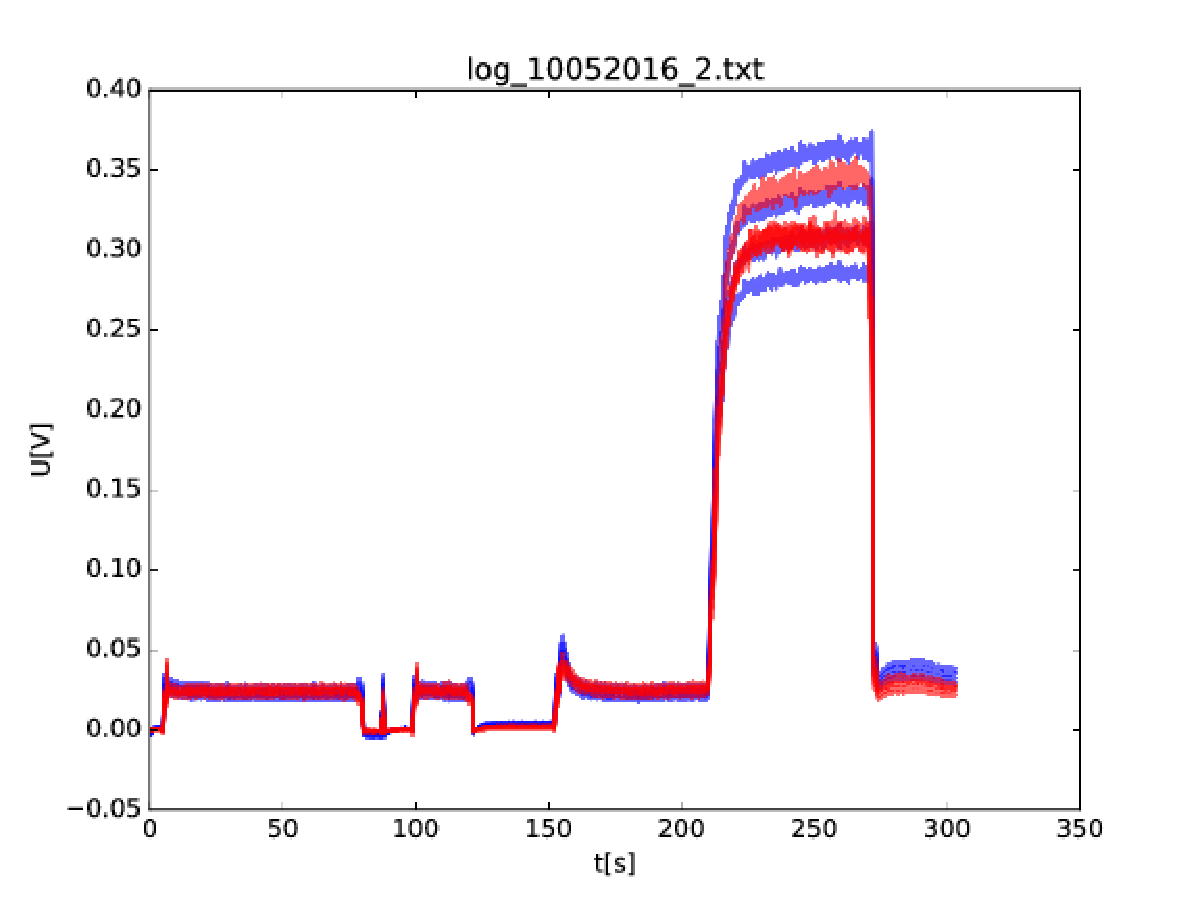
\includegraphics[width=\textwidth]{images/feed_switch.pdf} 
		\caption{feed switch}
	\end{center}
\end{figure}

\begin{figure}
	\begin{center}
		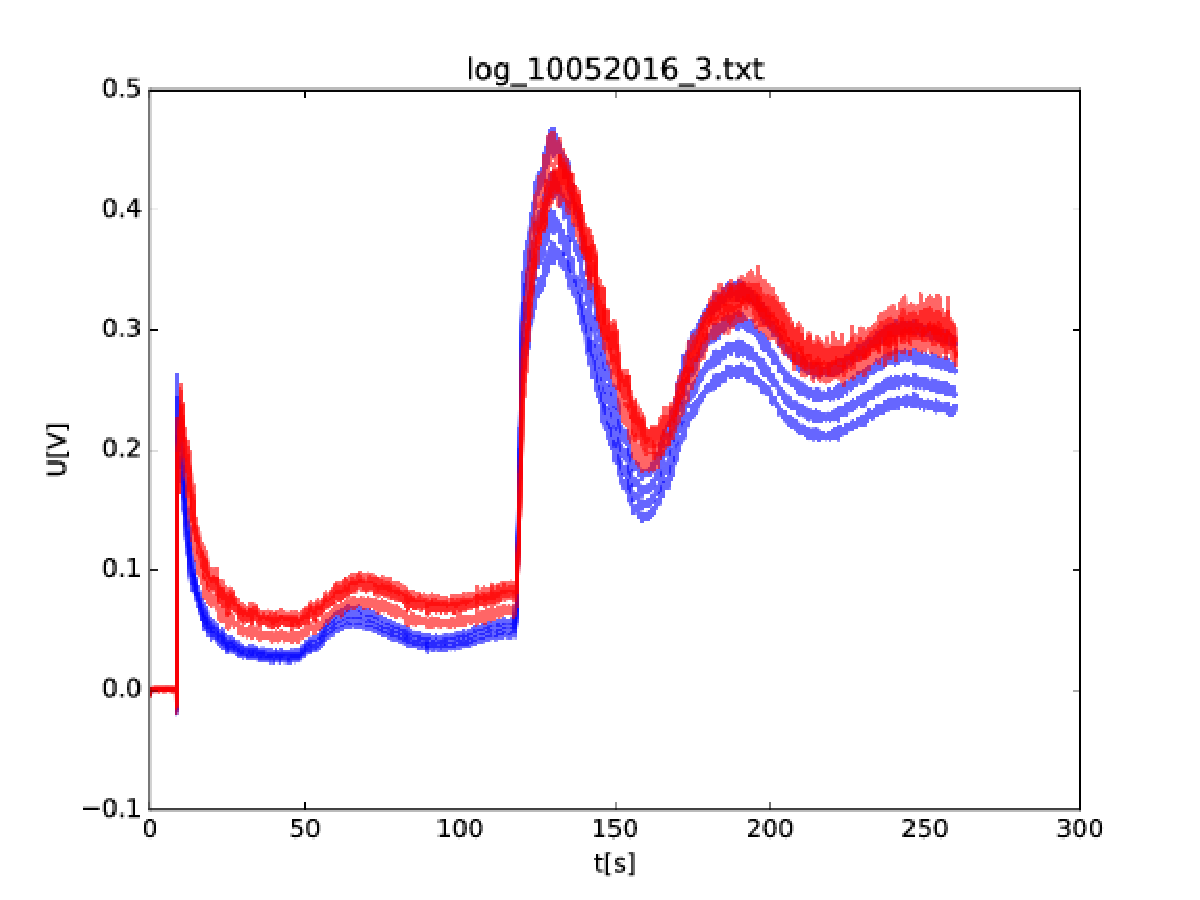
\includegraphics[width=\textwidth]{images/feed_add.pdf} 
		\caption{feed add}
	\end{center}
\end{figure}


